\documentclass{article}

\usepackage{ctex}
\usepackage{tikz}
\usetikzlibrary{cd}

\usepackage{amsthm}
\usepackage{amsmath}
\usepackage{amssymb}

%\usepackage{unicode-math}


\usepackage[textwidth=18cm]{geometry} % 设置页宽=18

\usepackage{blindtext}
\usepackage{bm}
\parindent=0pt
\setlength{\parindent}{2em} 
\usepackage{indentfirst}


\usepackage{xcolor}
\usepackage{titlesec}
\titleformat{\section}[block]{\color{blue}\Large\bfseries\filcenter}{}{1em}{}
\titleformat{\subsection}[hang]{\color{red}\Large\bfseries}{}{0em}{}
%\setcounter{secnumdepth}{1} %section 序号

\newtheorem{theorem}{Theorem}[section]
\newtheorem{lemma}[theorem]{Lemma}
\newtheorem{corollary}[theorem]{Corollary}
\newtheorem{proposition}[theorem]{Proposition}
\newtheorem{example}[theorem]{Example}
\newtheorem{definition}[theorem]{Definition}
\newtheorem{remark}[theorem]{Remark}
\newtheorem{exercise}{Exercise}[section]

\newcommand*{\xfunc}[4]{{#2}\colon{#3}{#1}{#4}}
\newcommand*{\func}[3]{\xfunc{\to}{#1}{#2}{#3}}

\newcommand\Set[2]{\{\,#1\mid#2\,\}} %集合
\newcommand\SET[2]{\Set{#1}{\text{#2}}} %


\newcommand\slattice{\mathcal{S}}
\newcommand\lattice{\mathcal{L}}
\newcommand\eql[1]{\ensuremath\mathbf{Eq}~{#1}}




\begin{document}
\title{Lattice}
\author{枫聆}
\maketitle
\tableofcontents

\newpage
\section{Ordered Sets}

\begin{definition}
\rm {\color{red} Partially ordered set} is a system $\mathcal{P} = (P,\leq)$ where $P$ is a nonempty set and $\leq$ is a binary relation on $P$ satisfying,for all $x,y,z \in P,$
\begin{enumerate}
	\item \rm {\makebox[8cm][l]{$x \leq x,$} (reflexivity) }
	\item \rm {\makebox[8cm][l]{if $x \leq y$ and $y \leq x$,then $x=y,$} (antisymmetry)}
	\item \rm {\makebox[8cm][l]{if $x \leq y$ and $y \leq z$,then $x \leq z.$} (transitivity)} 
\end{enumerate}
\end{definition}

\begin{definition}
\rm $\mathcal{C}$ is a {\color{red} chain} if for every $x,y \in \mathcal{C}$,either $x \leq y$ or $y \leq x.$
\end{definition}

{\color{blue} chain上的元素都可以相互比较,所以它是totally ordered 或者 linearly ordered}.

\begin{definition}
\rm We say that $x$ is {\color{red} covered} by $y$ in $\mathcal{P}$,written $x \prec y$,if $x \leq y$ and there is no $z \in P$ with $x \leq z \leq y$.
\end{definition}

\begin{definition}
\rm {\color{red} Hasse diagram} for a finite partially order set $\mathcal{P}$: the elements of $P$ are represented by points in the plane, and a line is drawn from $a$ up to $b$ precisely when $a \prec b$.
\end{definition}

\begin{center}
% https://tikzcd.yichuanshen.de/#N4Igdg9gJgpgziAXAbVABwnAlgFyxMJZARgBoAGAXVJADcBDAGwFcYkQAKM7gShAF9S6TLnyEUAJlLFqdJq3ZdpFPoOHY8BIuWmyGLNok47eAoSAwaxRbnvmHOZE6vOXRWlDol2Dinc7N1d3ESUgBmHwUjDn8VQIsRTRCpbxp9KMcKOLUEqw9Q1LlfaJNs2RgoAHN4IlAAMwAnCABbJB0QHAgkKRAACxh6KHZIMDYcxpa2mk6kMJp+weGCMfMJ1sR2mcQyPoGhoxGV+qb1na2ANnm9pdH4taQAdmmuxABWK8WD5buTpAAWZ5Id67T7gb7jX6IS4dF7Ahb7MG3CGTRBzGH-D4Iw4-FFoi6Ym5HED3RA9LZPEFY8GrSFnF4U+GEnHrMkvAGUpn8Sj8IA
\begin{tikzcd}
                                                 & {(1,1,1)} \arrow[ld, no head] \arrow[d, no head] \arrow[rd, no head] &                                                  \\
{(0,1,1)} \arrow[rd, no head] \arrow[d, no head] & {(1,0,1)} \arrow[ld, no head] \arrow[rd, no head]                    & {(1,1,0)} \arrow[d, no head] \arrow[ld, no head] \\
{(0,0,1)} \arrow[rd, no head]                    & {(0,1,0)} \arrow[d, no head]                                         & {(1,0,0)} \arrow[ld, no head]                    \\
                                                 & {(0,0,0)}                                                            &                                                 
\end{tikzcd}
\end{center}

\begin{definition}
\rm Given a partially order set, $f$ is a {\color{red} order preserving map} satisfying the condition $x \leq y$ implies $f(x) \leq f(y)$.
\end{definition}

\begin{definition}
\rm Given two posets $(P,\leq_S)$ and $(Q,\leq_Q)$,an {\color{red} order isomorphism} from $(P,\leq_S)$ to $(Q,\leq_Q)$ is a bijective order preserving map.
\end{definition}

\begin{definition}
\rm Given two posets $(P,\leq_S)$ and $(Q,\leq_Q)$,an {\color{red} order embedding} from $(P,\leq_S)$ to $(Q,\leq_Q)$ is a both order-preserving and order-reflecting map that $x \leq y \iff f(x) \leq f(y)$.
\end{definition}

{\color{blue}相比order isomorphism而言稍微弱一点,不需要是一个surjective}.

\begin{definition}
\rm An {\color{red} ideal} $I$ of a partially ordered set $\mathcal{P}$ is a subset of the elements of $P$ which satisfy the property that if $x \in \mathcal{P}$ and exists $y \in I$ with $x \leq y$,then $x \in I$.
\end{definition}

{ \color{blue} 衍生自the ideal of ring,后面我们将会看见 the ideal of lattice}.

\begin{definition}
\rm Given an ordered set $\mathcal{P}=(P,\leq)$. The {\color{red} dual of $P$} is another poset $\mathcal{P}^d=(P,\leq^d)$ with the order relation defined by $x \leq^d y \iff y \leq x$. 
\end{definition}

\begin{definition}
\rm The dual notion of an ideal is called a {\color{red} filter} that $F$ is a subset of $P$ such $x \geq y \in F$ implies $x \in F$  
\end{definition}

{\color{blue} 类似的还有principle ideal和principle filter. 就是通过一个元素生成的}.

\begin{definition}
\rm The poset $\mathcal{P}$ has a {\color{red} maximum}(element) if there exists $x \in P$ such that $y \leq x$ for all $x \in P$.

An element $x \in P$ is {\color{red} maximal}	if there is no element $y \in  P$ with $x \leq y$ and $x \neq y$. 
\end{definition}

{\color{blue} maximum是一个名词表示最大值(greatest),maximal是一个形容词表示极大的意思. 在poset中可能不只有一个maximal element}.

\begin{lemma}
\rm The following are equivalent for an poset $\mathcal{P}$.

\begin{enumerate}
	\item Every nonempty subset $S \subseteq P$ contains an element minimal in $S$.
	\item $\mathcal{P}$ contains no infinite descending chain \[a_0 > a_1 > a_2 > \cdots.\]{\color{blue} 这里去掉等号是指$a_0 \neq a_1 \neq a_2 \neq \cdots$} 
	\item If \[a_0 \geq a_1 \geq a_2 \geq \cdots\] in $\mathcal{P}$,then there exists $k$ such that $a_n = a_k$ for all $n \geq k$.
\end{enumerate}
\end{lemma}

{\color{red} 这个lemma被称为descending chain condition(DCC). 对偶地也有ascending chain condition(ACC). original 'a partially ordered set $\mathcal{P}$ requires that all decreasing sequences in $\mathcal{P}$ become eventually constant'}.

\begin{proof}
(2) $\Rightarrow$ (3). 前提只存在finite descending chain. 假设(3)不成立,且$a_0 \geq a_1 \geq a_2 \geq \cdots$是infinite chain. 则对于任意的$k$,都能找到$n \geq k$使得$a_n \neq a_k$且$a_k \geq a_n$,那么$a_k > a_n$. 这样从$k=0,1,2,\cdots$开始我们每次都可以找到$a_{n_0} > a_{n_1} > \cdots$. 这样我们实际构造了一个infinite descending chain,这是和前提矛盾的. 若$a_0 \geq a_1 \geq a_2 \geq \cdots$是一个finite chain,它的最后一个元素显然是满足(3),这和假设是矛盾的. 

(3) $\Rightarrow$ (2). 也是分infinite chain和finite chain来讨论,finite是显然的,infinite的时候可以把它变成finite.

(1) $\Rightarrow$ (2). (1)前提满足下,假设(2)不成立,即$\mathcal{P}$存在infinite descending chain. 把这个chain上的所有元素取出来组成一个subset $S$,那么任取$a_k$都有$a_{k+1} \leq a_k$. 即找不到minimal.

(2) $\Rightarrow$ (1). (2)前提满足下,假设(1)不成立.  这里需要用一下{\color{blue} 选择公理}了,定义$S$上一个选择函数$\func{f}{S}{T}$,其中$T \subseteq S$. 让$a_0 = f(S)$,递归地定义对任意的$i \in \omega$有$a_{i+1} = f(\Set{s \in S}{s < a_i})$. 接下来让这个definition make sense,(2)前提下$S$是没有minimal, 所以$\Set{s \in S}{s \leq a_i}$不是empty set. 这样就找到了一个infinite descending chain,与假设矛盾.

(1) $\Rightarrow$ (2) $\Rightarrow$ (3).

(3) $\Rightarrow$ (2) $\Rightarrow$ (1).

{\color{blue} done well}!
\end{proof}

\begin{lemma}
\rm Let $\mathcal{P}$ be an poset satisfyint the DCC. If $\varphi(x)$ is statement such that
\begin{enumerate}
	\item $\varphi(x)$ holds for all minimal elements of $P$,and
	\item whenever $\varphi(y)$ holds for all $y < x$,then $\varphi(x)$ holds,
\end{enumerate}
then $\varphi(x)$ is true for every element of $P$.
\end{lemma}

{\color{blue} 这个lemma有点意思,如果对$P$上所有的minimal element $m$都有命题$\varphi(m)$成立, 且$\mathcal{P}$满足DCC. 那么再加上一个条件: 只要对任意元素$x \in P$,满足$y < x$都有$\varphi(y)$成立. 则对任意元素$x \in P$都有$\varphi(x)$成立}.

\begin{proof}
其实(1)是(2)的一个special case. 在(1)(2)hold的情况下,我们试想一下$\varphi(x)$没有被hold住的是哪些元素呢? 即对于某个$x$,存在$y < x$使得$\varphi(y)$没有被hold. 递归地,我们再去考虑这个$y$. 那么这里就存在一条descending chain在这里,由于$\mathcal{P}$是满足$DCC$,所以这个descending chain是infinite的. 这条chain的结尾显然是一个minimal element,但是它是满足$\varphi(x)$. 所以实际上是不存在这里的$x$不满足$\varphi(x)$. 
\end{proof}

\begin{definition}
\rm Let $\mathcal{P}$ be poset. Two elements $a$ and $b$ of $\mathcal{P}$ are called {\color{red} comparable} if $a \leq b$ or $a \geq b$. Otherwise, they are called {\color{red}incomparable}.
\end{definition}

{\color{blue} 元素的可比性}.

\begin{definition}
\rm An {\color{red} antichain} in $\mathcal{P}$ is a subset $A$ of $\mathcal{P}$ in which each pair of different element are incomparable.
\end{definition}

\begin{definition}
\rm Define the {\color{red} width} of an poset $\mathcal{P}$ by
$$
	w(\mathcal{P}) = \sup\Set{|A|}{\text{A is an antichain in $\mathcal{P}$}}
$$
where $|A|$ denotes the cardinality(集合的势) of $A$. 
\end{definition}


\begin{definition}
\rm We define the {\color{red} chain-covering-number} CCN $c(\mathcal{P})$ to be the least cardinal number k, such that $P$ is a union of $k$ chains(finite) of $P$, means $P = \bigcup C_i$
\end{definition}

{\color{blue} 另一种covering number,有趣}.

\begin{lemma}
Suppose $P = \bigcup C_i$ where $i \in I$,then $ w(\mathcal{P}) \leq |I|$.
\end{lemma}

\begin{proof}
因为$ |A \cap C_i| \leq 1 $ for $i \in I$. 也就是说你把$A$里面的元素分开塞到$C_i$上,每次都只能塞一个. 那么最多你可以每个$C_i$上都塞一个. 
\end{proof}

\begin{theorem}
\rm (Dilworth ,1950) Let $\mathcal{P}$ be a finite poset. $w(\mathcal{P})$ is width. Then $\mathcal{P}$ is a union of $w(\mathcal{P})$-chains.
\end{theorem}

\begin{proof}
TODO.
\end{proof}

\newpage
\section{Semilattices, Lattices and Complete Lattices}

\subsection{Semilattice}
\begin{definition}
\rm A {\color{red} semilattice} is an algebra $\mathcal{S} = (S,*)$ satisfying, for all $x,y,z \in \slattice$,
\begin{enumerate}
	\item $x * x = x,$
	\item $x * y = y *x,$
	\item $x*(y*z) = x*(y*z).$
\end{enumerate}
where $*$ is binary operator.
{\color{red} 换句话说semilattice就是一个idempotent commutative semigroup(幂等交换半群)}. 
\end{definition}

\begin{theorem}
\rm In a semilattice $\slattice$,define $x \leq y$ if $x * y = x$. Then $(S,\leq)$ is a poset in which every pair of elements has a greater lower bound.

Conversely,given an poset $P$ with that property,define $x * y = g.l.b(x,y).$ Then $(P,*)$ is a semilattice.
\end{theorem}

\begin{proof}
先证明这个是一个poset. 
\begin{enumerate}
	\item $x * x = x$ implies $x \leq x,$
	\item if $x \leq y$ and $x \geq y$, then $x = x*y  = y*x = y,$
	\item if $x \leq y$ and $ y \leq z$. then $x *z = (x * y)*z = x *(y *z) = x * y = x$, so $x \leq z$.
\end{enumerate}
这个greater lower bound就是$x * y$. 首先证明它是一个lower bound,$x *(x*y)=x*y$ and $y*(x*y) = x*y$,所以$x*y$是一个lower bound. 再来证明所有的lower bound都比它小,假设$z \leq x$和$z \leq y$,即$z$是$\{x,y\}$的一个lower bound. 那么$z * (x * y) = z * y = z$,所以$z \leq (x*y)$. 最后$x*y$的一个greater lower bound. 
\end{proof}

{\color{blue} semilattice上弄了一个特殊的poset出来, 它最好的性质就是任意两个元素都有一个下确界}.

\begin{definition}
\rm A semilattice with the above ordering is usually called {\color{red} meet semilattice}. 对偶地,使得$x \geq y \iff x * y = x$,则称$\slattice$为是一个{\color{red} join semilattice}. 自然地在$(S,\leq)$下任意的pair都有一个least upper bound $x \vee y$.
\end{definition}

\begin{definition}\rm A {\color{red} homomorphism} between two semilattice is a map $\func{f}{\slattice}{\mathcal{T}}$ with the property that $f(x*y) = f(x) * f(y)$. An {\color{red} isomorphism} is a homomorphism that injective and surjective.

{\color{red} 一个semilattice homomorphism肯定是一个monotone function(相对于poset来说),但是一个monotone function并不一定是一个homomorphism}.
\end{definition}

{\color{blue} nothing new}... {\color{red} has some!}

\begin{definition}
\rm A semilattice is {\color{red} bounded} if there is a top/bottom element. 
\end{definition}



\begin{theorem}
\rm Let $\slattice$ be a meet semilattice. Define $\func{\phi}{S}{\mathcal{O}(S)}$ by
$$
\phi(x) = \Set{y \in S}{y \leq x}
$$
where $\mathcal{O}(S)$ is collection of all order ideals of $\slattice$. Then $\slattice$ is isomophic $(\mathcal{O}(S),\cap)$(注意这里是$\slattice$的image).
\end{theorem}

{\color{blue} 怎么感觉这些ideal都是principle ideal}.

\begin{proof}
$\cap$表示set inclusion,$\phi$是order-preserving和order-reflecting还是比较obvious. 所以$\phi$是一个order embedding of $\slattice$ into $\mathcal{O}(\slattice)$. Moreover $\phi(x \wedge y) = \phi(x) \cap \phi(y)$ because $x \wedge y$ is the greate lower bound of $\{x,y\}$,so that $z \leq x \wedge v$ if and only if $z \leq x$ and $z \leq y$. 
\end{proof}


\newpage
\subsection{Lattice}
\begin{definition}
\rm A {\color{red} lattice} is an algebra $\lattice = (L,\wedge,\vee)$ satisfying,for all $x,y,z \in L,$
\begin{enumerate}
	\item $x \wedge x = x$ and $x \vee x = x,$
	\item $x \wedge y = y \wedge x$ and $x \vee y = y \vee x,$
	\item $x \wedge (y \wedge z) = (x \wedge y) \wedge z$ and $x \vee (y \vee z) = (x \vee y) \vee z,$
	\item $x \wedge (x \vee y) = x$ and $x \vee (x \wedge y) = x.$ 
\end{enumerate}
\end{definition}

{\color{blue} 就第四个在我们眼里似乎没有那么自然,它叫absorption laws(吸收律),它在这里可以保证后面$\wedge$和$\vee$定义了相同的partial order(虽然是dual). 前三个我们知道lattice同时在两种binary operator都是semilattice,所以我们只要在lattice上定义前面合适的partial order,它就是both meet and join semilattice}. 

\begin{theorem}
\rm In a lattice $\lattice$,define $x \leq y$ if and only if $x \wedge y = x$. Then $(L,\leq)$ is a poset in which every pair of elements has a greatest lower bound and a least upper bound.  
\end{theorem}

\begin{proof}
给定一个pair $(x,y)$. 前面已经证明了$x \wedge y$是它的一个greater lower bound. 再根据lattice definition的第四条的第一个式子,$x \vee y$是它的一个upper bound,第二式子说明当$x \geq y$时,有$x \vee y = x$,对偶地$x \vee y$是least upper bound. 

这里若$x \wedge y = x$,则$x \vee y = (x \wedge y) \vee y = y$.  类似地$x \vee y = y$,则$x \wedge y = x \wedge (x \vee y) = x$.  所以有一个很重要的结论就是{\color{blue} $x \wedge y = x \iff x \vee y = y$}.
\end{proof}

{\color{red} 类似的我们可以通过一个poset构造lattice}.

\begin{theorem}
\rm Given an poset $\mathcal{P}$ with that above property,define $x \wedge y = \sup\{x,y\}$ and $x \vee y = \inf\{x,y\}$. Then $(P,\wedge,\vee)$ is a lattice.
\end{theorem}


{\color{blue} 所以实际上lattice可以有两种定义第一种是前面的代数定义,第二种就是在poset上定义join和meet操作,这一点要清楚}.


{\color{red} the definitions of sublattice,homomorphism and isomorphism )}.

\begin{definition}
\rm Two lattice $\lattice_1$ and $\lattice_2$ are {\color{red} isomorphic} if there is {\color{red} bijective} $\alpha$ from $\lattice_1$ to $\lattice_2$ such that for every $a,b$ in $\lattice_1$ the following two equations hold: $\alpha(a \wedge b) = \alpha(a) \wedge \alpha(b)$ and $\alpha(a \vee b) = \alpha(a) \vee \alpha(b)$. Such an $\alpha$ is called by an {\color{red} isomorphism}.  
\end{definition}

{\color{red} 在用poset基础上定义的lattice之间的isomorphism也可以用下述定理来描述}.

\begin{theorem}
\rm Two lattices $\lattice_1$ and $\lattice_2$ are isomorphic iff there is a bijection $\alpha$ from $\lattice_1$ to
$\lattice_2$ such that both $\alpha$ and $\alpha^{-1}$ are {\color{red} order-preserving}. 
\end{theorem}

\begin{proof}
如果$\alpha$是$\lattice_1$到$\lattice_2$的一个isomorphism和$a \leq b$ hold in $\lattice_1$. $a \leq b$ hold means $a = a \wedge b$,那么$\alpha(a) = \alpha(a \wedge b) = \alpha(a) \wedge \alpha(b)$,所以$\alpha(a) \leq \alpha(b)$. 反过来$\alpha^{-1}$也是一个isomorphism,所以$\alpha^{-1}$也是order-preserving的.

反过来如果$\alpha$是bijective的且$\alpha$和$\alpha^{-1}$都是order-preserving的. 给定$a,b \in \lattice_1$,有$a \leq a \vee b$,那么$\alpha(a) \leq \alpha(a \vee b )$. 同理对$b$也有$\alpha(b) \leq \alpha(a \vee b)$,那么$\alpha(a) \vee \alpha(b) \leq \alpha(a \vee b)$. 我们要把这个小于等于换成等于,就是要证明$\alpha(a \vee b)$确实是一个greatest upper bound,那么对应任意的upper $u$,即$\alpha(a) \vee \alpha(b) \leq u$,分别有$\alpha(a) \leq u$和$\alpha(b) \leq u$. 由于$\alpha^{-1}$也是order-preserving,所以有$a \leq \alpha^{-1}(u)$和$b \leq \alpha^{-1}(u)$,那么$a \vee b \leq \alpha^{-1}(u)$,在用$\alpha$作用一遍$\alpha(a \vee b) \leq u$. 到这里证明了$\alpha(a \vee b)$确实是一个greatest upper bound,即$\alpha(a) \vee \alpha(b) = \alpha(a \vee b)$. 同理也可以证$\alpha(b) \wedge \alpha(b) = \alpha(a \wedge b)$.
\end{proof}

\begin{example}
\rm 记录一个$\alpha$是bijective但只有$\alpha$ order-preserving,这样的$\alpha$可能不是一个isomorphism. Hasse图可能画的不标准!
\begin{center}
% https://tikzcd.yichuanshen.de/#N4Igdg9gJgpgziAXAbVABwnAlgFyxMJZARgBoAGAXVJADcBDAGwFcYkR6QBfU9TXfIRTlSxanSat2AI268QGbHgJEATKVXiGLNohABjOXyWCiZAMxbJukFCML+yocgCsFKzvacexgSpRuYjTaUnqyPg4m-q4aHqEG9op+zm6WwdbsdlziMFAA5vBEoABmAE4QALZIIiA4EEgALDQAFjD0dohgzIyMNDj0WIzsFfRocHX2ZZVIZLX1iG4gre1IXT19A0N6I2MTEVNViOpzSABsLW0da721m8Oj4-X75YfmffMA7Bcrnd03-YN7rsnvIDtV3jNvh1wAQ2M9pogahMjlD2JAwHDQS9ISdEG8lpc0bDJtiUbj8ctoejMSVSU1cYtKUSMSSEYtkecCT8YSz4YdOcivlyqcTslwgA
\begin{tikzcd}
                                              & a \arrow[rrrr, maps to] \arrow[ld, no head] \arrow[rdd, no head] &                                            &  &  & a \arrow[d, no head] \\
b \arrow[rrrrr, maps to] \arrow[rdd, no head] &                                                                  &                                            &  &  & b \arrow[d, no head] \\
                                              &                                                                  & c \arrow[rrr, maps to] \arrow[ld, no head] &  &  & c \arrow[d, no head] \\
                                              & d \arrow[rrrr, maps to]                                          &                                            &  &  & d                   
\end{tikzcd}
\end{center}
\end{example}

\begin{definition}
\rm If $\lattice$ is lattice and $L' \neq \emptyset$ is a subset of $L$ such that for every pair of elements $a,b in L'$ both $a \wedge b$ and $a \vee b$ are in $L'$,where $\wedge$ and $\vee$ are the lattice operations of $\lattice$,then we say $L'$ with the same operations of $\lattice$ is a {\color{red} sublattice} of $\lattice$. 
\end{definition}

\newpage
\subsection{Complete Lattice}
{\color{red} 集合的upper bound和 lower bound}.
\begin{definition}
\rm For a subset $A$ of a poset $P$,let $A^u$ denote the set of all upper bounds of $A$,
$$
\begin{aligned}
A^u &= \Set{x \in P}{x \geq a\ \text{for all}\ a \in A} \\
	&= \bigcap\limits_{a \in A} \uparrow a
\end{aligned}
$$
where $\uparrow a = \Set{x \in P}{x \geq a}$. Dually,$A^l$ is the set of all lower bounds of $A$,
$$
\begin{aligned}
A^l &= \Set{x \in P}{x \leq a\ \text{for all}\ a \in A} \\
	&= \bigcap\limits_{a \in A} \downarrow a
\end{aligned}	
$$
where $\downarrow a = \Set{x \in P}{x \leq a}$.
\end{definition}

思考一个问题{\color{red} poset $P$的一个subset $A$什么时候least upper bound}? 很显然$A^u$ 一定不是空的,更确切地说$A^u$有一个greatest lower upper $z$,而且$z \in A^u$,根据$z$的definition它是$A$的least upper bound. 这种情况下我们就说{\color{red} the join of $A$ exists,and write $z = \bigvee A$}. 对偶地,{\color{red} 考虑$A$的greatest lower bound},则$A^l$一定不为空,那么$A^u$里面是有一个lower upper bound的$w$,根据$w$的definition它是$A$的greatest lower bound. 这种情况下我们就说{\color{red} the meet of $A$ exists,and write $w = \bigwedge A$}.


\begin{theorem}
\rm Let $\slattice$ be a finite meet semilattice with greatest element 1. Then $\slattice$ is a lattice with join operation defined by 
$$
x \vee y = \bigwedge \{x,y\} ^u = \bigwedge (\uparrow x \cap \uparrow y).
$$
\end{theorem}

\begin{proof}
$\slattice$有greatest element,则$A^u$肯定不是空了,至少这个greatest element里面. $\bigwedge A^u$就是要找$A^u$的lower upper bound. 由于$\slattice$是一个finite lattice,所以$A^u$也是finite. $A^u$里面的元素做有限次meet操作得到就是一个lower upper bound,但是你还得说明它在$A^u$里面. 这是很显然的,$x \wedge z_1 \wedge \cdots \wedge z_k = x$其中$z_i \in A^u$,所以$\bigwedge A^u$是它的一个upper bound.

还得proof一下它是一个lattice,上面只是证明了这个东西是well behaved. Lattcie definition中前三条还是比较明显的.
$$
x \wedge (x \vee y) = x
$$
这也很显然,因为$x \vee y \in \{x,y\}^u$.
$$
x \vee (x \wedge y) = x
$$
因为$x \wedge y$是$\{x,y\}$的一个greatest lower bound,有$x \geq x \wedge y$,那么$\inf(x,x \wedge y) = x$.
\end{proof}

这个theorem告诉我们: {\color{red} if a finite poset $P$ has a greatest element and every pair of elements has a meet,
then $P$ is a lattice}. 这就是lattice非代数形式的definition.

\begin{theorem}
\rm Every finite subset of a lattice has a greatest lower bound and a leaset upper bound.
\end{theorem}

\begin{proof}
$\lattice$是finite,则它的subset也是finite. 前面我们知道lattice中任意一个pair都有greatest lower bound和least upper bound,这是meet和join定义下的partial order所带来的性质. 在finite subset里面先挑两个出来做meet或者join可以得到inf和sup它们也是属于$L$的,再从剩下的subset里面再挑一个出来做同样的操作,这个操作只会做有限多次,所以最终我可以得到这个subset的greatest lower bound和least upper bound.
\end{proof}

{\color{red} 这个性质在infinite lattice下可能就无法成立,自然地completely就arised}.

\begin{definition}
\rm Given poset $\lattice$. If every subset $A$ of $\lattice$ has a greatest lower bound $\bigwedge A$ and a least upper bound $\bigvee A$,then $\lattice$ is called {\color{red} complete lattice}. 
\end{definition}

%{\color{red} finite lattice是complete的,并且所有complete lattice都包含greatest element和least element}.

\begin{definition}
\rm a {\color{red} complete meet semilattice} is an poset $\slattice$ with greatest element and the property that every nonempty subset $A$ of $S$ has a greatest lower bound $\bigwedge A$.
\end{definition}

%{\color{red} 下面这个theorem让我们抛弃了更强的finite,如何在complete meet semilattice上构造一个complete lattice出来}.

\begin{theorem}
\rm If $\lattice$ is a complete meet semilattice,then $\lattice$ is a complete lattice with the join operation defined by
$$
\bigvee A = \bigwedge A^u = \bigwedge (\bigcap\limits_{a \in A} \uparrow a).
$$
\end{theorem}

\begin{proof}
和前面在finite meet semilattice上构造lattice类似,这里finite换成了complete. 这里我们直接就可以知道在$A^u$非空时,$\bigwedge A^u$是有意义的,并且这里有$1 \in A^u$. 那么$\bigwedge A$的definition是满足$A$的least upper bound.
\end{proof}

\newpage
\subsection{Closure System}

{\color{blue} 这一章我们的主旋律.
\begin{center}
% https://tikzcd.yichuanshen.de/#N4Igdg9gJgpgziAXAbVABwnAlgFyxMJZARgBoAGAXVJADcBDAGwFcYkQAdDnGADx2ABjRpmYAnGAAI4ATzg8AtgF8QS0uky58hFACZSxanSat2XHvyEi44qRDQwx9HBDEq1G7HgJFyBowwsbIic3HwCwqISkmLMjPDuRjBQAObwRKAAZmIQCkh+IC5IxB4g2blI+oUQ+aXleYhk1ZU0ABYw9FBIYHGMNDj0WIzskGBsSpRKQA
\begin{tikzcd}
                                & \text{closure system} \arrow[rd] &                                    \\
\text{closure rules} \arrow[ru] &                                  & \text{closure operator} \arrow[ll]
\end{tikzcd}
\end{center}
}
\begin{definition}
\rm A {\color{red} closure system} on a set $X$ is a collection $\mathcal{C}$ of subsets of $X$ thats is closed under arbitrary intersections(任意的交). The sets in $\mathcal{C}$ are called closed set. 
\end{definition}

\begin{example}
\rm 有一些closure system的例子
\begin{enumerate}
	\item closed subsets of topological space,
	\item subgroups of group,
	\item subspace of vector space.
	\item convex subsets of euclidean space $\mathbb{R}^n$,
	\item order ideals of an poset.
\end{enumerate}
\end{example}

{\color{red} By convention,特殊地$\bigcap \emptyset = X$ ( $\bigwedge (A\cup\emptyset) = \bigwedge A \vee \bigwedge \emptyset = \bigwedge A$,这就是在说它$\bigwedge \emptyset$比任意子集都大),closure system现在就是complete meet semilattice with greatest element $X$,所以你按前面构造定义出join,那么closure system就是一个complete lattice了}.


\begin{definition}
\rm A {\color{red} closure} operator on a set $X$ is a map $\func{\Gamma}{\mathfrak{P}(X)}{\mathfrak{P}(X)}$ satifying, for all $A,B \subseteq X$,
\begin{enumerate}
	\item $A \subseteq \Gamma(A),$
	\item $A \subseteq B$ implies $\Gamma(A) \subseteq \Gamma(B),$
	\item $\Gamma(\Gamma(A)) = \Gamma(A).$
\end{enumerate}
\end{definition}

%{\color{blue} closure的general definition有点意思}. 简单地来说,就是(1)集合的闭包包含集合本身;(2)如果两个集合有包含关系,则它们的闭包也有相同的包含关系;(3)闭包的闭包是其本身.

{\color{red} 如何在$X$上利用已知的closure system构造一个closure operator}?

\begin{theorem}
\rm If $\mathcal{C}$ is a closure system on a set $X$,then the map $\func{\Gamma_{\mathcal{C}}}{\mathfrak{B}(X)}{\mathfrak{B}(X)}$ defined by 
$$
\Gamma_{\mathcal{C}}(A) = \bigcap \Set{D \in \mathcal{C}}{A \subseteq D}
$$
is a closure operator. Moreover $\Gamma_{\mathcal{C}}(A)=A$ if and only if $A \in \mathcal{C}$
\end{theorem}

%{\color{red} 所有包含这个集合的closed set的交是这个集合的closure}. {\color{blue} 在topology里面closure是包含这个集合最小的closed set}. 

\begin{definition}
\rm A set of {\color{red} closure rules} on a set $X$ is a collection $\sum$ of properties $\varphi(S)$ of subsets of $X$. where each $\varphi(S)$ has one of the forms
$$
x \in S
$$
or 
$$ 
Y \subseteq S \Rightarrow z \in S
$$ 
with $x,z \in X$ and $Y \subseteq X$. A subset $D$ of $X$ is said to be closed with respect to these rules if $\varphi(D)$ is true for each $\varphi \in \sum$.
\end{definition}

{\color{blue} 你看到这里一定会感觉非常的困惑,抽象的closure rules到底是个啥东西?不急接着往下看你终会明白的}.

\begin{example}
\rm 对应前面列举到的closure system.
\begin{enumerate}
	\item In topological space, all rules $Y \subseteq S \Rightarrow z \in S$ where $z$ is an accumulation point of $Y$.  
	\item In subgroup, the rule $1 \in S$ and all rules
	$$
		\begin{aligned}
			x \in S &\Rightarrow x^{-1} \in S
			\{x,y\} \in S &\Rightarrow xy \in S
		\end{aligned}
	$$
	\item In vector space,$0 \in S$ and all rules $\{x,y\} \subseteq S \Rightarrow ax + by \in S$ with $a,b$ scalars. 
\end{enumerate}
\end{example}

{\color{blue} closure rules就是一系列判断closed set的命题}.

\begin{theorem}
\rm {\color{red} If $\Gamma$ is a closure operator on a set $X$},$\sum_{\Gamma}$ be the set of (1)all rules where $c \in \Gamma(\emptyset)$,and (2)all rules
$$
Y \subseteq  S \Rightarrow z \in S
$$
with $z \in \Gamma(Y)$. Then a set $D \subseteq X$ satisfies all the rules of $\sum_\Gamma$ if and only if $\Gamma(D) = D$.
\end{theorem}

\begin{proof}
(1)是在说$\emptyset$的image非空?(2)是在说取$S$上任意子集$Y$,都有$\Gamma(Y) \subseteq S$. 直觉上就说这群规则是一个closure rule,满足它的只有closed set,自然地在closure operator上也是一个closed set. 可这条件都TM都abstract nosense了!!!

我尝试用closure operator的definition来推一下,$Y \subset S$,结合前面那么有
$$
Y \subseteq \Gamma(Y) \subseteq S.
$$
特殊点,把$Y$换成$S$,有$S \subseteq \Gamma(S) \subseteq S$,所以$\Gamma(S) = S$. 但是(1)在这里有啥用啊?保证$S$非空?

反过来若$\Gamma(D) = D$. 自然地,当$Y \subseteq D$,则有$Y \subseteq \Gamma(Y) \subseteq \Gamma(D) =  D$.
\end{proof}

{\color{blue} 当有一个closure operator之后,最重要是我们知道了closed set在它的作用下是它本身}.

\begin{theorem}
\rm {\color{red} If $\sum$ is a set of closure rules on set $X$},let $\mathcal{C}_{\sum}$ be the collection all subsets of $X$ that satisfy all the rules of $\sum$. Then a set $\mathcal{C}_{\sum}$ is a closure system. 
\end{theorem}

\begin{proof}
这个定理可以更形象地去理解closure rule到底是什么? 假设$A,B$是满足$\sum$里面所有rules的两个集合. 我们看它们的交,对于第一类规则$x \in S$,很显然在交下是保持的,因为$x \in A$和$x \in B$,则$x \in A \cap B$. 对于第二类的规则,若$C \subseteq A \cap B$,且它是某个规则里面对应的$Y$,那么$C \subseteq A$和$C \subseteq B$,对应地有某个$z \in A$和$z \in B$,所以$z \in A\cap B$. 综上$A \cap B$也是属于$\mathcal{C}_{\sum}$.
\end{proof}

{\color{blue} 在这里我们才终于认识到这样closure rules这样抽象的东西,它确实可以刻画一堆closed set组成了一个closure system}.

{\color{red} 总结一下前面的所有东西,前面提到过一个closure system其实是一个complete lattice,现在我们多了另外两个概念closure operator和closure rules. 我们前面3个定理就是在说明它们之前是可以相互转换的,例如给定一个closure operator,它$\Gamma(D) = D$可以对应上closure rules,然后我们用closure rules刻画的sets收集起来,这些sets在交运算下也能保持封闭,所以这些sets是一个closure system,最终也得到了complete lattice}. {\color{blue} 后面我们用$\mathcal{C}_\Gamma$ 表示由closure operator $\Gamma$ 生成的closed sets($\Gamma(D)=D$) with set inclusion 构成poset}. 很自然地有下面的定理.

\begin{theorem}
\rm If $\Gamma$ is a closure operator on a set $X$,and {\color{red} the operations on $\mathcal{C}_\Gamma$} are given by 
$$
\begin{aligned}
\bigwedge\limits_{i \in I} D_i &= \bigcap\limits_{i \in I} D_i \\
\bigvee\limits_{i \in I} D_i &= \Gamma(\bigcup\limits_{i \in I} D_i).
\end{aligned}
$$
in where $D_i \in \mathcal{C}_{\Gamma}$. Then $\mathcal{C}_\Gamma$ is complete lattice.
\end{theorem}

\begin{proof}
由Theorem 2.25和Theorem 2.26可以知道一族closed set $\mathcal{C}_{\Gamma}$是一个closure system. 自然地我们要用集合上union和interestion. 先考虑interestion $\bigcap\limits_{i \in I} D_i$,它确实是greatest lower bound,且在closure system interestion下有
$$
\Gamma(\bigcap\limits_{i \in I} D_i) = \bigcap\limits_{i \in I} D_i.
$$
所以$\bigcap\limits_{i \in I} D_i \in \mathcal{C}_{\Gamma}$. 对于union $\bigcup\limits_{i \in I} D_i$,它肯定是$X$上的greatest upper bound,但是它不一定在$\mathcal{C}_{\Gamma}$中,所以我们要在$\mathcal{C}_{\Gamma}$中找所有包含它的closed sets,再交一下就可以得到$\mathcal{C}_{\Gamma}$上的greatest upper bound. 这是我们的思路,假设这样的closed sets为$\{A_j\}_{i \in J}$. 明显地,$\bigcup\limits_{i \in I} D_i \in \bigcap \{A_j\}_{i \in J}$. 我们只要证明$\Gamma(\bigcup\limits_{i \in I} D_i) \subseteq A_j$对任意地$j \in J$都成立即可,即它是$\mathcal{C}_{\Gamma}$包含$\bigcup\limits_{i \in I} D_i$最小的closed set. 但是证明过于简单2333,直接用closure operator第二个定义即可. 因为$\bigcup\limits_{i \in I} D_i \subseteq A_j$,所以$\Gamma(\bigcup\limits_{i \in I} D_i) \subseteq \Gamma(A_j) \subseteq A_j$. 
\end{proof}

略{\color{red} algebra一般定义和subalgebra上的closure operator}.

下面是一个{\color{red} representation theorem,刚才是closure operator 到 complete lattice,现在是complete lattice到 closuse}.

{\color{blue} 下面的定理在说任意一个complete lattice和一些closed set构成lattice同构}.

\begin{theorem}
\rm If $\lattice$ is a complete lattice,define a closure operator $\Delta$ on $L$ by
$$
\Delta(A) = \Set{x \in L}{x \leq \bigvee A}.
$$
Then {\color{red} $\lattice$ is isomorphic to $\mathcal{C}_{\Delta}$}. The isomorphism $\func{\varphi}{\lattice}{\mathcal{C}_{\Delta}}$ is just given by $\varphi(x) = \downarrow x$.
\end{theorem}

\begin{proof}
$\Delta$是一个closure operator还是比较obvious. 我们来回顾一下$\downarrow x$的definition $\downarrow x = \Set{y \in L}{ y \leq x}$,所以$\Delta(\downarrow x) = \downarrow x \in \mathcal{C}_{\Delta}$.

先证bijective,若对于$x,y \in L$有$\varphi(x) = \varphi(y)$,那么$y \in \varphi(x)$和$x \in \varphi(y)$,就有$y \leq x$和$x \leq y$,所以$x = y$,即$\varphi$是injective. 任意一个$C \in \mathcal{C}_{\Delta}$,那么都有least upper bound $u \in C$. 自然地$\varphi(u) = C$,即$\varphi$是surjective.

给定任意地$x,y \in L$,那么
$$
\varphi(x \wedge y) = \uparrow (x \wedge y) = \uparrow x \cap \uparrow y = \varphi(x) \wedge \varphi(y).
$$
同理
$$
\varphi(x \vee y) = \uparrow (x \vee y) = \uparrow x \cap \uparrow y = \varphi(x) \vee \varphi(y).
$$
综上$\varphi$是一个isomorphism.
\end{proof}


{\color{blue} 换句话说就是$q$如果是join irreducible,则它不可能是其他某些元素的一个join}. 

\begin{definition}
\rm An element $q$ of lattice $\lattice$ is called {\color{red} join irreducible} if $q = \bigvee F$ for a {\color{red} finite set} $F$ implies $q \in F$. The set of all join irreducible elements in $\lattice$ is denoted by $J(\lattice)$.
\end{definition}

{\color{red} 如果$\lattice$有一个最小元素0,那么0其实不是join irreducible的,因为$0 = \bigvee \emptyset$. 如果想要把0含进来,特殊地$J_0(\lattice) =J(\lattice) \cap \{0\}$. 当然还有一种定义如果$q$是join irreducible,那么当$q = r \vee s$,则$q = r$或者$q =s$,在这种定义下$q$已经是针对非空的集合来说的}. 

\begin{lemma}
\rm If a lattice $\lattice$ satisfies the DCC,then every element of $\lattice$ is a join of finitely many join irreducible elements.
\end{lemma}

\begin{proof}
用反证法来证明: 假设存在$\lattice$上一些元素,使得找不到join irreducible elements的join正好是它们. 我们把这些元素记为集合$S$,根据DCC $S$里面有一个最小值,我们设为$x$. 那么$x$肯定也不是join irreducible的,如果它是的话,它就是它自己的一个join,那么$x \notin S$. 既然$x$不是一个join irreducible,那么有$x = \bigvee F$其中$F$是一个finite set且里面的元素都是严格小于$x$的,由于$x$是最小元素这个概念,所以比它小的元素都是the join of finitely many join irreducible elements. 那么对于$F$而言,任意的$f \in F$都有一个$G_f \subseteq J(\lattice)$的join是$f$. 所以
$$
x = \bigvee\limits_{f \in F}\bigvee G_f.
$$
这里$f = \bigvee G_f$,所以$x$可以表示称有个多个join irreducible elements的join,这就矛盾了. 这里应该还要考虑一下$x = 0$,但是讨论0确实没什么意义,0可以定义为join irreducible也可以不是,这里还是避免这种情况吧...
\end{proof}

\begin{definition}
\rm An element $q$ of a complete lattice $\lattice$ is said to be {\color{red} completely join irreducible} if $q = \bigvee X$ implies $q \in X$ for {\color{red} arbitrary (possibly infinite) subsets} $X \subseteq L$. Let $J^*(\lattice)$ denote the set of all completely join irreducible elements of $\lattice$. 
\end{definition}

\begin{proposition}
\rm In general,$J^{*}(L) \subseteq J(L)$,but for lattices satisfying the ACC,equality holds.
\end{proposition}

\begin{proof}
每个completely join irreducible element肯定是 join irreducible   element. 这是很自然地,它是任意多个元素的join,那肯定可以挑出来有限多个元素 with $q$的join还是$q$. ACC有了之后,$\lattice$上任意非空的子集都有一个最大元素,那么我们现在假设一个join irreducible element $x$它不是complete的,即可以找到某个集合$S$,有$x = \bigvee S$且$x \notin S$. 矛盾就来了,ACC下least upper bound应该是在$S$里面,所以现在又有每个join irreducible element是completely join irreducible.
\end{proof}


{\color{blue} 满足ACC和DCC的lattice一个表示方法}.

\begin{theorem}
\rm Let $\lattice$ be a lattice satisfying the ACC and DCC. Let $\sum$ be the set of all closure rules on $J(L)$ of the form
$$
F \subseteq S \Rightarrow q \in S
$$
where $q$ is join irreducible,$F$ is a finite subset of $J(L)$,and $q \leq \bigvee F$. (Include the degenerate cases $p \in S \Rightarrow q \in S$ for $q \leq p$ in $J(\lattice)$.) Then $\lattice$ is isomorphic to the lattice of $\mathcal{C}_{\sum}$ of $\sum$-closed sets.
\end{theorem}

\begin{proof}
这里同构证明用isomorphism definition下面那个定律,即bijective加两个order-preserving. 那么先给出两个order-preserving的map $\func{f}{\lattice}{\mathcal{C}_{\sum}}$和$\func{g}{\mathcal{C}_{\sum}}{\lattice}$
$$
\begin{aligned}
f(x) &= \downarrow x \cap J(\lattice)\\
g(S) &= \bigvee S.
\end{aligned}
$$
需要证明它们两个互为逆映射(感觉好突兀啊,虽然原文中说straightforwrad233333). 那么对于$gf(x) = x$,前面那个lemma应该告诉我们了,在DCC下$\lattice$每一个元素都是a join of finitely many join irreducible elements对应是$f(x)$的操作. 

那么对于$fg(S) = S$,在ACC下$\bigvee S \in S$,也就是我们可以找到一些finite set $F \subseteq S$使得$\bigvee F = \bigvee S$,按照closure rules,所有join irreducible $q \leq \bigvee F$都是属于$S$的,$f(\bigvee F)$就是在做这件事. 但是这样得到是不是全部的$S$呢? 考虑其他finite set $F'$, 那么$\bigvee F' \leq \bigvee S = \bigvee F$,$f$是order-preserving的,所以有$f(\bigvee F') \subseteq f(\bigvee F)$,所以$f(\bigvee F)$涵盖了整个$S$.
\end{proof}

{\color{blue} 按照下面定义$x$明显是一个upper bound,但是条件更强它还要是一个least upper bound,dense 稠密在这里还是很形象,$x$就是一个划分}.

\begin{definition}
\rm A subset $Q$ of a complete lattice $\lattice$ is {\color{red} join dense} if for every $x \in L,$
$$
x = \bigvee\Set{q \in Q}{q \leq x}.
$$
\end{definition}

{\color{blue} fixed point来表征complete lattice}.

\begin{theorem}
\rm A lattice $\lattice$ is complete of if and only if every order-preserving map $\func{f}{\lattice}{\lattice}$ has a fixed point.
\end{theorem}

\begin{proof}
($\Rightarrow$) 如果给定一个 complete lattice $\lattice$和一个order-preserving map $\func{f}{\lattice}{\lattice}$. 定义集合$A = \Set{x \in L}{f(x) \geq x}$. 注意到$0 \in A$ (0表示minimal element of $L$). 再让$a = \bigvee A$,那么对于任意的$x \in A$都有$a \geq x$,结合$f$是order-preserving我们有
$$
f(a) \geq \bigvee\limits_{x \in A} f(x)  \geq \bigvee\limits_{x \in A} x = a.
$$
所以$a \in A$,即$f(a) \geq a$,两边再作用一下$f$有$f^2(a) \geq f(a)$,这说明$f(a) \in A$. $a$可是整个$A$的join,那么有$a \geq f(a)$. 综上$f(a) = a$,$a$就是这个fixed point.

($\Leftarrow$) 这个方向的证明略微有些复杂,{\color{blue} 故事主线是在every order-preserving map has a fixed point的前提下,假设$\lattice$不是complete,然后构造出来出来一个order-preserving map没有fixed point造成矛盾}.

假设$\lattice$不是complete,那么先给出第一个claim.

\textbf{Claim 1}: $\lattice$没有最大元素1或者存在一个chain $C \subseteq L$满足ACC且没有meet(supermum).

证这个claim,我们还是用反证法,{\color{blue} 假设$\lattice$有最大元素1和所有满足ACC的chain $C \subseteq L$都有meet}. 我们仔细考虑一下这个假设,先回顾一下我们前面关于complete meet semilattice的definition,是要有一个poset满足有greatest element并且所有非空的子集都有meet,然后我们可以通过这个complete meet semilattice构造出来一个complete lattice,我们的证明大体上也是这个思路,但是使用其对偶的形式(因为你可以观察到我们假设的第二个条件有些不一样),即在complete join semilattice来构造,从而制造了一个contradiction.

考虑某个子集$S$的所有upper bound $S^u$. {\color{blue} 注意到$1 \in S^u$},所以$S^u$不是emptyset. 我们再来定义一个poset $\mathcal{P}$,它是$S^u$上所有满足ACC的chains的一个collections. $\mathcal{P}$上的partial-order定义为若$C_1 \leq C_2$则$C_1$是$C_2$的一个filter(我们回顾一下filter的定义,它是ideal的对偶形式,即首先有$C_1 \subseteq C_2$,若$x \geq y \in C_1$则$x \in C_1$其中$x \in C_2$).

我们再来考虑这个特殊的poset $\mathcal{P}$上的chain (chain of chains),任取$\mathcal{P}$上的一个chain $\{C_i\}_{i \in I}$,那么$\bigcup\limits_{i \in I} C_i \in \mathcal{P}$,根据上面定义的partial order这是显然的,而且$\bigcup\limits_{i \in I} C_i$它是这个chain的一个upper bound. 根据Zorn's lemma,$\mathcal{P}$上有一个maximal element $C_m$. {\color{blue} 根据我们的假设$C_m$满足ACC是有meet的},这个meet我们用$a$来表示,即$\bigwedge C_m = a$. 很明显$a$在是$S$的一个upper bound,所以$a \in S^u$. {\color{blue} 我们现在来证明$a = \bigwedge S^u$}(至于为什么后面你就知道了),还是用反证法(23333),假设$a$不是$S^u$的greatest lower bound,那么存在$t \in S^u$,使得$a \nleq t$. 则有$a \wedge t \in S^u$,为什么呢?因为任取$s \in S$,都有$s \wedge (a \wedge t) = s$. 自然地$a > a \wedge t$(严格大于没有等号),那么chain $C_m \cup \{a \wedge t\}$也是满足ACC,且大于$C_m$,这就矛盾了,所以$a = \bigwedge S^u = \bigvee S$. 

所以我们证明了对于任意的$S \subseteq L$都有join,那么马上我们有
$$
\bigwedge S = \bigvee S^l.
$$
所以$S$的meet也有意义了,但是这里$S^l$我们不知道是不是非空的啊? 注意最前面我们用0加上complete join semilattice来构造complete lattice,但是我们这里不需要构造因为lattice是给定了,那么对于任意非空的$S$,$\bigwedge S \in S^l$的,所以$S^l$也是非空的,这里没有问题. 综上$\lattice$是一个complete lattice与前提矛盾. \textbf{Claim 1}证闭.

原谅我这个证明写不去了,原文省略太多的东西了...
\end{proof}

{\color{red} 来另一个1955年给出的第一个证明}.

\begin{lemma}
如果$\lattice$是incomplete,那么存在两个chain $C$和$D$满足下面条件,
\begin{enumerate}
	\item $C$是一个strictly ascending chain(严格大于),$D$是一个strictly descending chain(严格小于).
	\item $D$中的每个元素都严格大于$C$中的每个元素.
	\item 不存在$a \in L$使得它同时是$C$的upper bound和$D$的lower bound. 
\end{enumerate}
\end{lemma}

\begin{proof}
Proof of above lemma.
\end{proof}

\begin{proof}
这里我们还是证if every preserving map $\func{f}{\lattice}{\lattice}$ has a fixed point then $\lattice$ is complete. 还是假设$\lattice$是incomplete,然后我们构造一个preserving map没有fixed point.

假设$C,D$是满足前面lemma的两个chains. 然后我们来定义这个特殊的preserving map $f$,对于任意的$x \in \lattice$,我们可以分两种情况来看,{\color{blue} $x$是$D$的lower upper或者不是}. 

第一种情况若$x$是$D$的lower upper,反过来那么它肯定不是$C$的upper bound,那么肯定存在某些$c \in C$满足$c \nleq x$. 我们把这些$c$记为
$$
C(x) = \Set{c \in C}{c \nleq x}.
$$
这种情况下我们取$f(x) = \min C(x)$,即$C(x)$中的最小值.

第二种情况$x$不是$D$的lower upper,那么肯定存在某些$d \ D$满足$c \ngeq x$. 我们把这些$d$记为
$$
D(x) = \Set{d \in D}{d \ngeq x}.
$$
这种情况下我们取$f(x) = \max D(x)$,即$D(x)$中的最大值.

这种情况定义出来的$f(x)$都会满足$f(x) \ngeq x$或者$f(x) \nleq x$,所以是不存在$f(x) = x$,即没有fixed point的.

接下来我们证明$f$是一个preserving map,取$x \leq y$. 我们分下面几种情况来分别说明:
\begin{enumerate}
	\item $x$是$D$的lower bound,$y$是$D$的lower bound. 那么$f(x) = \min C(x)$和$f(y) = \min C(y)$. 若$y \ngeq c$,则$ x \ngeq c$ (else $y \geq x \geq c$),所以$C(y) \subseteq C(x)$.
	\begin{center}
	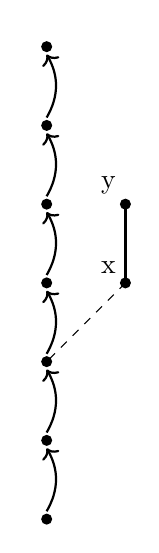
\begin{tikzpicture}
    \fill (0,0) circle (2pt) node[above left](a) {};
	\fill (0,-1) circle (2pt) node[above left](b) {};
	\fill (0,-2) circle (2pt) node[above left] {};
	\fill (0,-3) circle (2pt) node[above left] {};
	\fill (0,-4) circle (2pt) node[above left] {};
	\fill (0,-5) circle (2pt) node[above left] {};
	\fill (0,-6) circle (2pt) node[above left] {};
	\fill (1,-3) circle (2pt) node[above left] {x};
	\fill (1,-2) circle (2pt) node[above left] {y};
	\draw[->,thick] (0,-6+0.1) to [bend right] (0,-5-0.1);
	\draw[->,thick] (0,-5+0.1) to [bend right] (0,-4-0.1);
	\draw[->,thick] (0,-4+0.1) to [bend right] (0,-3-0.1);
	\draw[->,thick] (0,-3+0.1) to [bend right] (0,-2-0.1);
	\draw[->,thick] (0,-2+0.1) to [bend right] (0,-1-0.1);
	\draw[->,thick] (0,-0.9) to [bend right] (0,-0.1);
	\draw[thick] (1,-3) -- (1,-2);
	\draw[dashed] (1,-3) -- (0,-4);
	\end{tikzpicture}
	\end{center}
	$C$是一个升链,那么$C(x)$可以想象成这条链上一堆点,那么$C(x)$还是一个升链,$C(y)$是它的一个子集必然满足$\min C(x) \leq \min C(y)$,则$f(x) \leq f(y)$.
	\item $x$是$D$的lower bound,$y$不是$D$的lower bound. 那么$f(x) = \min C(x)$和$f(y) = \max D(y)$,显然$f(x) \leq f(y)$.
	\item $x$不是$D$的lower bound,$y$是$D$的lower bound. 这是不可能的,因为$x \leq y$,那么当$y$是$D$的lower bound的时候,$x$也是$D$的lower bound.
	\item $x$不是$D$的lower bound,$y$不是$D$的lower bound. 那么$f(x) = \max D(x)$和$f(y) = \max D(y)$. 若$x \nleq d$,则$y \nleq d$ (else $x \leq y \leq d$). 所以$D(x) \subseteq D(y)$. 由于$D(y)$是一个降链上点的集合,这个集合还是一个降链,你在降链上找子集$D(x)$,肯定有$\max D(x) \leq \max D(y)$,则$f(x) \leq f(y)$.
\end{enumerate}
综上$f(x) \leq f(y)$总是成立,所以$f$确实是一个preserving map.
\end{proof}

%https://core.ac.uk/download/pdf/4886291.pdf complete lattice上的endomorphim monotone map不动点构成集合是还是一个complete lattice.

\newpage
\section{Alegbraic Lattices}

\subsection{Algebraic Closure Operators}


\def\temp{&} \catcode`&=\active \let&=\temp
% https://tikzcd.yichuanshen.de/#N4Igdg9gJgpgziAXAbVABwnAlgFyxMJZABgBpiBdUkANwEMAbAVxiRAB12cYAPHYAMYNMTAE4wABBDQxRdHBFEBfEEtLpMufIRQAWclVqMWbTtz7BGAcxgAjOVgEShI8VJlyFy1epAZseAREZADMhvTMrIgcXLz8AhAAtmgMMNwSDPJ4AjAqahoB2kT6YdQRJtFmcZYMNvZ0jhlZjrk+BVpBKGQAbOHGUTHm-DgAFpKZONmSEABmzsJwMFASizh5vv4dOsj6vWX9prEWo+PNOVJzLovLq3mGSzYIKKAzoklIZCAKSABM+5GHWwwKxYMCWURyACeSmADAYSk4AHE6IlEnQABQAQQAlBJOAB3B6SJEotHogBCuIkADIALwSPHsZGojE4xkCOhoRnMsmUxmcbmk1m4zg0GDEplCilUumCllY9lMLmUzgwMBQcFQlTUTJAhgABU0gR0IFEWCsIxwbRAr3eiE+30QAEZ-hUYjzhRJ6ZxbOaBEq5WSAGK4kA6uh6w2FTogVIzK35G1vRJIF1fCBIEKugY+4GgzV0aGw+Ek+VsglEwMYvmyqtYkXsDlc0u8hsClue0Xius172SsuK5XY1XqgvQsOxiMwA1GorROMJ3y2lOIP7ppD6IwAypHfhYWCMeauaYeeSKdHWOwOAS42x0a5SMASAAknDRow5DGAABklM-tZOkazjGZoWouLzJr81COlmW5ulUxxjCsaQXM4SRoHQAg4BI04wIkao4HAEhYERABWECghIsBgIsAG6tOUZbGwC7WsumbQRmiAAKzZocQzAPuMCHlcYgnrIZ6iBetRXg0N4SHeD4EC+b7yCMn4-koAB6Aj-hO9EztGJosYmbGIJujo8XBOb9mSbJ9r6Vj+s2NkYiGEh6VOBlMdEoGWqoFBKEAA
\begin{center}
\begin{tikzcd}
\text{closure operator} \arrow[ddd, "\begin{array}{ll}\Gamma(A) \wedge \Gamma(B)  &=  \Gamma(A) \cap \Gamma(B) \\ \Gamma(A) \vee \Gamma(B)  &= \Gamma(A \cup B)\end{array}"'] \arrow[rrrr, "\Gamma(A) = \bigcup \Gamma(F) "] &  &  &  & \text{algebraic closure operator} \arrow[ddd, "\begin{array}{ll}\Gamma(A) \wedge \Gamma(B) &=  \Gamma(A) \cap \Gamma(B) \\ \Gamma(A) \vee \Gamma(B) &= \Gamma(A \cup B)\end{array}"] \\
                                                                                                                                                                                                                             &  &  &  &                                                                                                                                                                                      \\
                                                                                                                                                                                                                             &  &  &  &                                                                                                                                                                                      \\
\text{complete lattice} \arrow[ddd, "\text{ideal closure operator(algebraic) based on $\mathcal{L}$}"'] \arrow[rrrr, "\text{the set of compact elements is join dense}"]                                                     &  &  &  & \text{algebraic lattice} \arrow[ddd, "\text{ideal closure operator(algebraic) based on $\mathcal{L}^c$}"]                                                                            \\
                                                                                                                                                                                                                             &  &  &  &                                                                                                                                                                                      \\
                                                                                                                                                                                                                             &  &  &  &                                                                                                                                                                                      \\
\text{the lattice of closed set} \arrow[rrrr, "\Gamma(A) = \bigcup \Gamma(F) "']                                                                                                                                             &  &  &  & \text{the lattice of closed set}                                                                                                                                                    
\end{tikzcd}
\end{center}

\begin{definition}
\rm A {\color{red} closure operator} $\Gamma$ on a set $X$ is said to be {\color{red} algebraic} if for every $B \subseteq X$,
$$
\Gamma(B) = \bigcup \SET{\Gamma(F)}{$F$ is finite subset of $X$}.
$$
\end{definition}

\begin{definition}
\rm Let $\lattice$ be a complete lattice. An element $x \in L$ is {\color{red} compact} if whenever $x \leq \bigvee A$, then there exists a finite subset $F \subseteq A$ such that $x \leq \bigvee F$. The set of all compact elements of $\lattice$ is denoted by $\lattice^c$
\end{definition}

{\color{blue} 这里的compact就是在说如果$x$小于$A$,则$x$小于$A$中的部分元素. 这个定义看起来还是比较自然的}.

\begin{proposition}
\rm $\lattice^c$ is closed under finite joins and contains 0,so it is a join semilattice with a least element.
\end{proposition}

\begin{proof}
假设$x$和$y$是两个compact元素,集合$A$表示such $x \vee y \leq A$. 那么自然地有$x \leq x \vee y \leq A $和$y \leq x \vee y \leq A$,所以各自都可以找到$x \leq F_x \subseteq A$和$y \leq F_y \subseteq A$. 从$F_x$和$F_y$各挑一个元素出来$a$和$b$出来,那么$x\vee y \leq a\vee b$. 0属于$\lattice^c$这是很自然的,它比任何一个元素都小.
\end{proof}

\begin{definition}
\rm A lattice $\lattice$ is said to be {\color{red} algebraic, or compactly generated}, if it is complete and $\lattice^c$ is join dense in $\lattice$, i.e., $x = \bigvee (\downarrow x \cap L^c)$ for every $x \in L$.
\end{definition}

{\color{blue} 换句话说就是在$\lattice^c$中比$x$小的元素它们的join是$x$,每一个$x$都可以划分$\lattice^c$. 另外一个理解就是任意$x \in L$,都是某些compact elements的join,这就是为什么说compactly generated}.

\begin{example}
\rm 自然地,finite lattice都是algebraic lattice, 首先finite lattice是complete lattice,其中每一个元素都是compact,所以有$\lattice = \lattice ^c$,那么$x = \bigvee (\downarrow x \cap L) = \bigvee (\downarrow x) = x$,即$\lattice$是join dense的. 
\end{example} 

\begin{example}
\rm 一个complete lattice并一定是一个algebraic lattice:
\begin{enumerate}
	\item 区间$[0,1]$上所有的实数和自然序构成一个complete lattice $\mathcal{K}$,那么$\mathcal{K}^c = {0}$,但是它并不是join dense的. 
	\item 下面的Hasse图也是complete lattice,但是$z$并不是一些complete element的join,那么$\lattice ^c$就不是join dense的.
	\begin{center}
	\begin{tikzpicture}
	 \usetikzlibrary{positioning}
		\tikzset{mynode/.style={draw,circle,inner sep=1.5pt,outer sep=0pt}
	}
    \node [mynode,label=above:{$z$}] (z) at (0,0) {};
    \node [mynode] (a) at (2,2) {};
    \node [draw,circle,fill,inner sep=0.5pt] (dd) at (2.7,0.94) {};
    \node [draw,circle,fill,inner sep=0.5pt] (dd) at (2.5,1.26) {};
    \node [draw,circle,fill,inner sep=0.5pt] (dd) at (2.3,1.6) {};
    \node [mynode] (b) at (2.9,0.6) {};
    \node [mynode] (c) at (3,0) {};
    \node [mynode] (d) at (2.9,-0.68) {};
    \node [mynode] (e) at (2.7,-1.36) {};
    \node [mynode] (f) at (2,-2) {};
    
    \draw (z) -- (a)
    	  (b) -- (c)
    	  (c) -- (d)
    	  (d) -- (e)
    	  (z) -- (f)
    	  (e) -- (f);
    	 
	\end{tikzpicture}
	\end{center}
\end{enumerate}

\begin{definition}
\rm A closure rule is said to be {\color{red} finitary} if it is a rule of the form $x \in S$ or the form $F \subseteq S \Rightarrow  z \in S$ with $F$ a finite set.
\end{definition}

\begin{theorem}
\rm {\color{red} (algebraic和finitary的关系)} A closure operator $\Gamma$ is algebraic if and only if $\Gamma = \Gamma_{\sum}$ for some set $\sum$ of finitary closure rules.
\end{theorem}

\begin{proof}
若$\Gamma$是一个$X$上的algebraic closure operator,我们要构造一组finitary closure rules来描述它的closed sets. 那么我们规定 {\color{red} 若$S \subseteq X$是closed 当且仅当对任意的finite set $F \subseteq S$都有$\Gamma(F) \subseteq S$}. 我们再来证明这个断言的正确性,正向是比较明显的,反过来要证明$S$是一个closet set即$\Gamma(S) = S$,在$\Gamma$的作用下,已经有$S \subseteq \Gamma(S)$,所以我们只需要证明$\Gamma(S) \subseteq S$. 因为$\Gamma$是algebraic的,所以对于finite set $F \subseteq S$,有$\Gamma(S) = \bigcup \Gamma(F)$,结合前提有$\bigcup \Gamma(F) \subseteq S$,那么$\Gamma(S) \subseteq S$. 我们由已经证明的结论构造出一族closure rules它们是finitary: 对任意的finite set $F \subseteq S \Rightarrow z \in S$其中$z \in \Gamma(F)$. 这族closure rules对应的closed set就是$\Gamma$上所决定的. 

前面命题的正向是在描述一个represention,那么反过来$\Gamma_{\sum}$到底在这里是什么意思呢?在确定closure rules情况下,我们就确定了$X$上的closed sets,随即它们构成了一个closure system,在之前closure system那一章,我们已经证明了,那么我们再在这个closure system上构造一个closure operator $\Gamma_{\sum}$定义如下
$$
\Gamma_{\sum}(A) = \bigcap \Set{S \in \mathcal{C}_{\sum}}{ A \subseteq S}
$$
其中$\mathcal{C}_{\sum}$表示closure rules确定的closed set. 是不是感觉绕了一个大湾?哈哈. whatever its done!

反过来如果$\sum$是一族finitary closure rules,可以得到上述定义的closure operator $\Gamma_{\sum}$,现在我们要来说明它是algebraic. 你得证明$\Gamma_{\sum}(B)$是$B$靠着closure rules生成的. 这里的证明去看universe alegbra中证明$\text{Sg}$是一个algebraic closure operator的方法.
\end{proof}

\newpage
\begin{theorem}
\rm {\color{red} (在algebraic closure operator上构造algebraic lattice)} Let $\Gamma$ be an algebraic closure operator on set $X$. Then $\mathcal{C}_\Gamma$ is an algebraic lattice whose compact elements are $\SET{\Gamma(F)}{$F$ is a finite subset of $X$}$.
\end{theorem}

\begin{proof}
首先我们得说明$\mathcal{C}_\Gamma$是一个complete lattice. 给定一族$\mathcal{C}_\Gamma$上的元素$B_{i \in I}$,我们定义$\bigvee\limits_{i \in I} B_i = \Gamma(\bigcup\limits_{i \in I} B_i)$和$\bigwedge_{i \in I} B_i = \Gamma(\bigcap_{i \in I} B_i)$,其中最大元是$\Gamma(X)$和最小元是$\Gamma(\emptyset)$. 所以$\mathcal{C}_{\Gamma}$是一个complete lattice.


给定$X$上的有限子集$F$和$X$上子集族$A_{i \in I}$. 若$\Gamma(F) \leq \bigvee\limits_{i\in I}\Gamma(A_i) = \Gamma(\bigcup\limits_{i\in I} A_i)$,要{\color{red} 证明$\Gamma(F)$是compact的,就是要证明$\Gamma(F) \subseteq \bigvee\limits_{j \in J} \Gamma(A_j)$其中$J$是有限的且$J \subseteq I$}.

由于$\Gamma$是algebraic的,那么
$$
F \subseteq \Gamma(F) \subseteq \Gamma(\bigcup\limits_{i\in I} A_i) = \bigcup\SET{\Gamma(G)}{$G$ is finite subset of $\bigcup\limits_{i\in I} A_i$}.
$$
对于任意的$x \in F$,都存在$x \in \Gamma(G_x)$,那么
$$
\Gamma(F) \subseteq \Gamma(\bigcup\limits_{x \in F}\Gamma(G_x)).
$$
实际上若$G$是$\bigcup\limits_{i\in I} A_i$的有限子集,那么$G \subseteq \bigcup\limits_{j\in J} A_j$,所以
$$
\Gamma(F) \subseteq \Gamma(\bigcup\limits_{x \in F}\Gamma(G_x)) \subseteq \Gamma(\bigcup\limits_{x \in F} \Gamma(\bigcup\limits_{j\in J_x} A_j)) = \bigvee\limits_{x \in F} \bigvee\limits_{j\in J_x} \Gamma(A_j) = \bigvee\limits_{\begin{aligned} x &\in F \\ j &\in J_x \end{aligned}} \Gamma(A_j).
$$

反过来,若$C$是$\mathcal{C}_{\Gamma}$上的compact element. {\color{red}我们要证明$C$是$X$上某个有限子集的闭包}. 因为$C$是closed的,则$\Gamma(C) = C$. 再由$\Gamma$是algebraic的,那么$C = \bigcup\SET{\Gamma(F)}{$F$ is finite subset of $C$}$. 又因为$C$是compact的,所以存在有限多个$\Gamma(F_1),\cdots,\Gamma(F_n)$使得$C = \Gamma(F_1) \vee \cdots \vee \Gamma(F_n) = \Gamma(F_1 \cup \cdots \cup F_n).$命题得证.

{\color{red} 最后证明$\mathcal{C}_{\Gamma}^c$是join dense的}. 对于任意的$B \in \mathcal{C}_{\Gamma}$,$B$是closed,那么$B = \bigvee\limits_{i \in I} \Gamma(F_i)$其中finite subset $F \subseteq B$ (这里已经可以说明$B$是compactly generated).  自然地有$\bigvee(\downarrow B \cap \mathcal{C}_{\Gamma}^c) \leq A$且$\Gamma(F_i)_{i \in I} \in \mathcal{C}_{\Gamma}^c$,那么$\bigvee(\downarrow B \cap \mathcal{C}_{\Gamma}^c) = B$. 命题得证.

\color{blue} 我们用algebraic closure operator生成了一个algebraic lattice,其上每一个元素都是compact elements的join,自然地联想到closure operator是algebraic的那个条件,每一个closed set都可以用finitely generated closed set来表示.
\end{proof}


\begin{definition}
\rm If $\Gamma$ is a closure operator on $X$ and $B$ is closed subset of $X$, then we way a set $A$ is a {\color{red} generating set} for $B$ if $\Gamma(A) = B$. The Set $B$ is {\color{red} finitely generated} if there is a finite generating set for $B$.  The set $A$ is {\color{red} minimal generating set} for $B$ if $A$ generates $B$ and no proper subset of $A$ generates $B$.
\end{definition}

\begin{corollary}
\rm Let $\Gamma$ be an algebraic closure operator on $X$. Then the finitely generated subset of $X$  are precisely the compact elements of $\mathcal{C}_{\Gamma}$.
\end{corollary}

\begin{example}
\rm 若$\mathcal{C}_{\Gamma}$是algebraic的,则$\Gamma$不一定是algebraic,也就是说$\Gamma$生成的lattice 是algebraic的,但是$\Gamma$本身不一定是algebraic. 下面举一个列子.

例如定义$X = Y \cup \{b\}$其中$Y$是finite set,$X$表示为它们的disjoint union(不交并). 然后定义$X$上的closure operator $\Gamma$为: 若$A$是$Y$的一个proper set(真子集),则$\Gamma(A) = A$; 特别地$\Gamma(Y) = X$; 若$b \in B \subseteq X$,则$\Gamma(B) = X$. $\Gamma$一个well defined closure operator,可以验证一下. 那么$\Gamma$生成的closed set为$Y$的所有proper set和$X$,它们构成的lattice $\mathcal{C}_{\Gamma}$是和$Y$上所有子集构成的lattice $\lattice_{\mathfrak{P}(Y)}$是isomorphic,这个isomorphism是比较明显的,$Y$上的proper set映到它本身,$X$映到$Y$.  $Y$是一个finite set,所以$\lattice_{\mathfrak{P}(Y)}$是一个algebraic lattice,{\color{red} 有个问题那么isomorphism是保持algebraic的?这个是显然的},想想就行. 考虑$\Gamma(Y)$,其中$b \in \Gamma(Y)$,但是对任意的$F \subseteq Y$都有$b \notin \Gamma(F)$,所以$\Gamma(Y)$是不满足$\Gamma$是algebraic的.
\end{example} 

\newpage 
\begin{definition}
\rm Let $\slattice = (S, \vee)$ be a join semilattice. A subset $A$ of $S$  is called an {\color{red} ideal} if
\begin{enumerate}
	\item $x,y \in A$ implies $x \vee y \in A$. 
	\item if $z \leq y \in A$ impiles $z \in A$.
\end{enumerate}

{\color{blue} 用自然语言来描述就是ideal首先是要在$\vee$的作用下封闭的. 若存在对任意一个元素$z$,它小于等于ideal中的某个元素,那么$z$也在ideal里面}.
\end{definition}

\begin{proposition}
\rm {\color{red}(ideal closure operator的引入)} Ideals are defined by closure rules,so the intersection of a set of ideals of $\slattice$ is again one. Since the closure rules are finitary, {\color{red} the lattice of ideals is algebraic}. 

The closure operator $I$ on $S$ such that $I(B)$ is the ideal of $\slattice$ generated by $B$ is given by
$$
I(B) = \SET{x \in S}{$x \leq \bigvee F$ for some finite $F \subseteq B$}.
$$
The ideal lattice of a join semilattice is denoted by $\mathcal{I}(\mathcal{S})$. The ideal lattice of a lattice $\lattice$ is likewise denoted by $\mathcal{I}(\lattice)$.    
\end{proposition}

{\color{blue} 不得不说closure rules抽象却深刻,扮演了一个很重要的角色}.

\begin{proof}
{\color{red} 我们来证明$I$是一个closure operator且$I(B)$是一个ideal}. 

任取$x,y \in I(B)$,那么分别对应存在$x \leq F_x$和$y \leq F_y$,自然地$x \vee y \leq \bigvee(F_x \cup F_y)$其中$F_x$和$F_y$都是finite的,所以$x \vee y \in I(B)$. 若$z \leq y \in I(B)$,那么$z \leq \bigvee F_y$,所以$z \in I$. 综上$I(B)$是一个ideal.  


$B \subseteq I(B)$,这是显然的,取每个$B$上单点集. 自然地$A \subseteq B$,也有$I(A) \subseteq I(B)$. 考虑$x \in I(I(B))$,那么存在finte set $F$对应$x \leq  \bigvee F \subseteq I(B)$. 自然地有$F \subseteq I(B)$,那么对于任意$y \in F$,都对应一个$ y \leq \bigvee F_y \subseteq B$. 所以
$$ 
F \leq \bigvee F \leq \bigvee \bigcup\limits_{y \in F} F_y.
$$
自然地$x \leq \bigvee \bigcup\limits_{y \in F} F_y.$所以$x \in I(B)$,即$I(B) \supseteq I(I(B))$,前面已经保证了$I(I(B)) \supseteq I(B)$,所以$I(I(B)) = I(B)$.

\end{proof}

\begin{theorem}
\rm {\color{red} (ideal closure operator生成的algebraic lattice的性质)} If $\slattice$ is a join semilattice with 0, then the ideal lattice $\mathcal{I}(\mathcal{S})$ is algebraic. The {\color{red} compact elements of $\mathcal{I}(\mathcal{S})$ are the principal ideals} $\downarrow x$ with $x \in S$. Conversely, if $\lattice$ is an algebraic lattice, then $\lattice^c$ is a join semilattice with 0, and $\lattice \cong \mathcal{I}(\lattice ^ c)$.
\end{theorem}

\begin{proof}
先来证明$\mathcal{I}(\slattice)$的compact elements是principle ideals. $I$是一个algebraic closure operator在上面已经证明了. 由Theorem 3.9我们知道compact element是$I(F)$其中$F$是$S$上的finite subset. 我们需要证明$I(F)$里面有一个maximal element,即$\bigvee F \in I(F)$. 由于$F$是finite的,前面的结论是显然的,所以$I(F) = \downarrow \bigvee F$.

如果$\lattice$是一个algebraic lattice,$\lattice^c$是一个join semilattice with 0 在proposition 3.3中已经证明了. 这里的$I$就是下面定理Theorem 3.16中$\Delta$更加朴素刻画,因为$I$在定义上可以更直观地看出它是algebraic的.

\end{proof}

\begin{theorem}
\rm {\color{red}(第一同构定理?)} If $\lattice$ is an algebraic lattice, define a algebraic closure operator $\Delta$ on the $\lattice^c$ by
$$
	\Delta(A) = \Set{x \in \lattice^c}{x \leq \bigvee A}
$$ 
where $A \subseteq \lattice^c$. Then $\lattice$ is isomorphic to $\mathcal{C}_\Delta$. Then isomorphism $\func{\varphi}{\lattice}{\mathcal{C}_\Delta}$ is just given by $\varphi(a) = \Set{x \in \lattice^c}{x \leq a}$.
\end{theorem}

\begin{proof}
$\Delta$是一个closure operator前面已经证明过了. 考虑$x \in \Delta(A)$,那么有$x \leq \bigvee A$. 由于$x$本身是$L$上的一个compact element,那么就可以找到一个有限子集$F \subseteq A$,使得$x \leq \bigvee F$,所以$\Delta(A) = \bigcup\limits_{x \in \Delta(A)} \Delta(F_x).$ 即$\Delta$是algebraic的.

先证bijective. 给定$a,b \in L$,若$\varphi(a) = \varphi(b)$,那么$a = \bigvee \varphi(a) = \bigvee \varphi(b) = b$,{\color{red} 注意两边等号成立的条件是$\lattice^c$是join dense(join dense终于在这里起作用了)},所以$\varphi$是injective. 对于任意的$C \in \mathcal{C}_\Delta$,它对应一个子集$A \subseteq \lattice^c$,使得$\Delta(A) = C$,那么我们取$a = \bigvee A$,我们知道compact element的join还是一个compact element,所以$a \in \lattice^c$,那么$\varphi(a) = C$,即$\varphi$是surjective.

再证homomorphism. 
$$
\begin{aligned}
\varphi(a \wedge b) = \varphi(a) \cap \varphi(b) = \varphi(a) \wedge \varphi(b) \\
\varphi(a \vee b) = \varphi(a) \cup \varphi(b) = \varphi(a) \vee \varphi(b).
\end{aligned}
$$

%{\color{blue} 从这个定理的证明里面,你可以发现从$\lattice^c$上构造一个algebraic closure operator出来,是不需要$\lattice^c$是join dense的这个条件,但是为了说明isomorphism才加上这个条件}.
\end{proof}	

\end{example}


\newpage
\begin{definition}
\rm A subset $D$ of an ordered set $\mathcal{P}$ is said to be {\color{red} \emph{up-directed}} if for every $x,y \in D$ there exists $z \in D$ with $x \leq z$ and $y \leq z$.
\end{definition}

\begin{example}
\rm Every chain, or more generally every join semilattice, forms an up-directed set.
\end{example}

\begin{theorem}
\rm Let $\Gamma$ be a closure operator on a set $X$. The following are equivalent.
\begin{enumerate}
	\item $\Gamma$ is an algebraic closure operator.
	\item The union of any up-directed set of $\Gamma$-closed sets is $\Gamma$-closed. 
	\item The union of any chain of $\Gamma$-clsoed sets is $\Gamma$-clsoed.
\end{enumerate}
\end{theorem}

\begin{proof}
(1) $\Rightarrow$ (2). 给定$\Gamma$是一个algebraic closure operator. 设$D \subseteq \mathcal{C}_{\Gamma}$上的一个up-directed set, {\color{red}那么若$C_1,C_2 \in D$,则存在$C_3 \in D$使得$C_1 \subseteq C_3$和$C_2 \subseteq C_3$}. (只有清楚了$D$的定义,接下来的事情就好办了)我们要证明$\bigcup D$也是一个closed set,那么自然地考虑$\Gamma(\bigcup D)$,由于$\Gamma$是algebraic的,所以
$$
\Gamma(\bigcup D) = \bigcup \Set{\Gamma(F)}{F\ \text{is finite subset of}\ \bigcup D}.
$$
我再来考虑这个$F$,换句话说$F \subseteq \bigcup\limits_{j \in J} C_j$,其中$C_j \in D$和$J$是finite的. 那么
$$
\Gamma(F) \subseteq \Gamma(\bigcup\limits_{j \in J} C_j). 
$$
由于$D$是一个up-directed set,所以存在某个$C_m > C_j$对任意的$j \in J$成立,那么
$$
\Gamma(\bigcup\limits_{j \in J} C_j) \subseteq \Gamma(C_m) = C_m \subseteq \bigcup D.
$$
所以对任意的$F$,都有$\Gamma(F) \subseteq \bigcup D$,那么$\Gamma(\bigcup D) \subseteq \bigcup D$,所以$\Gamma(\bigcup D) = \bigcup D$,即$\bigcup D$也是一个closed set.

(2) $\Rightarrow$ (3). 这个方向是trivial的,因为chain是一种特殊的up-directed set.

(3) $\Rightarrow$ (1). 给定$\Gamma$是$X$上的一个closure operator,且任意一个closed sets组成的chain的交还是一个closed set. 对于任意的$S \in X$,我们对$S$的基数$|S|$进行归纳,证明任意的$|S|$都有
$$
\Gamma(S) = \bigcup \Set{\Gamma(F)}{F\ \text{is finite subset of}\ \bigcup S}.
$$
当$|S|=1$时,这是显然的$F=S$. 假设$|S| = n$时上述等式成立,那么$|S| = n+1$时,让$S = W \cup \{a\}$,其中$|W| = n$. 那么
$$
\Gamma(S) = \Gamma(W \cup \{a\}) = \Gamma(W) \vee \Gamma(a) = \left( \bigcup\limits_{\text{finite}~F \subseteq W} \Gamma(F) \right) \vee \Gamma(a) = \left( \bigvee\limits_{\text{finite}~F \subseteq W} \Gamma(F) \right) \vee \Gamma(a)$$
(3)在这里怎么用呢? 感觉有点弱啊,似乎只能说明$\mathcal{C}_\Gamma$是complete的.
\end{proof}

\begin{definition}
\rm The lattice $\lattice$ is said to be {\color{red} weakly atomic} if whenever $a > b$ in $\lattice$, there exist elements $u,v \in L$ such that $a \geq u \succ v \geq b.$ ($\succ$ means cover)
\end{definition}

\begin{example}
\rm 所有的finite lattice都是weakly atomic的;闭区间$[0,1]$上所有实数自然序构成的lattice不是weakly atomic,给定一个$v$,你找不到它的cover $u$.
\end{example}

\begin{theorem}
\rm Every algebraic lattice is weakly atomic.
\end{theorem}

\begin{proof}
给定$\lattice$上任意两个元素$a,b$,若$a > b$, 那么存在一个compact element $c$使得$a \geq c$且,$b \nleq c$. 这是因为$\lattice$是compactly generated,所以$a$和$b$都是一些compact element的join,$a>b$则说明存在$a$对应的一些compact element是不小于等于$b$的. 接着我们考虑这样一个集合$Q=\Set{x \in a/b}{x \ngeq c}$ (其中$a/b$表示$b \leq x \leq a$称之为interval sublattice或者quotient sublattice). 注意到$Q$不是一个$\emptyset$,因为$b \in Q$. 我们考虑$\lattice$ 上所有的chains,任意一个chain的union还是在$Q$里面,假设这个union大于等于$c$,然而如果出现这种情况,这个chain肯定是infinite的,那么$c$小于等于finite subset of it,这就矛盾了. 根据Zorn's Lemma,$Q$存在一个maximal element $u$, 然后我们取$v = c \vee u$, $u$是covered by $v$,假设存在$u \leq z \leq v$,那么$z \ngeq c$,则$z \in Q$,这与$u$是maximal element是矛盾的. 这样我们就构造出来了满足weakly atomic的$u$和$v$,证毕. 
\end{proof}

\begin{definition}
\rm A lattice $\lattice$ is said to be {\color{red} upper continuous} if whenever $D$ is an up-directed set having a least upper bound $\bigvee D$, then for any element $x \in L$, the join $\bigvee_{d \in D}(a \wedge d)$ exists, and 
$$
a \wedge \bigvee D = \bigvee_{d \in D}(a \wedge d).
$$
The property of being lower continuous is defined dually.
\end{definition}

\begin{theorem}
\rm Every algebraic lattice is upper continuous.
\end{theorem}

\begin{proof}
给定$\lattice$是一个algebraic lattice和$D$是$\lattice$上一个up-directed subset. 显然地$\bigvee_{d \in D}(a \wedge d) \leq a \wedge \bigvee D$. 我们用$r = a \wedge \bigvee D$. 考虑$c \in \downarrow r \cap L^c$,自然地$c \leq r$,那么$c \leq a$和$c \leq \bigvee D$. 由于$c$是compact的,所以存在finite set $F \subseteq \bigvee D$使得$c \leq \bigvee F$,$D$又是up-directed,所以存在$e \in D$使得$\bigvee F \leq e$,那么$c \leq e$. 前面也有$c \leq a$,所以$c \leq a \wedge e$. 因此
$$
r = \bigvee (\downarrow \cap L^c) \leq \bigvee_{d \in D}(a \wedge d).
$$
所以有$a \wedge \bigvee D \leq \bigvee_{d \in D}(a \wedge d)$,综上$a \wedge \bigvee D = \bigvee_{d \in D}(a \wedge d)$. 
\end{proof}

\begin{definition}
\rm An element $a \in L$ is  called an {\color{red} atom} if $a \succ 0$, and a {\color{red} coatom} if $1 \succ a$. 
\end{definition}

\begin{definition}
\rm An element $q$ in a complete lattice $\lattice$ is {\color{red} completely meet irreducible} if, for every subset $S$ of $L$, $q  = \bigwedge S$ implies $q \in S$.
\end{definition}

\begin{definition}
\rm A {\color{red} decomposition} of an element $a \in L$ is a representation $a = \bigwedge Q$ where $Q$ is set of completely meet irreducible elements of $\lattice$
\end{definition}

\begin{definition}
\rm A lattice is {\color{red} strongly atomic} if $a>b$ in $\lattice$ implies there exists $u \in L$ such that $a \geq u \succ b$.
\end{definition}

\newpage
\section{Representation by Equivalence Relations}

{\color{red} 这章目的是像在群论里面那样每一个group都能找到和它同构的permutation group,同样每一个lattice也都能找到和它同构的equivalence relation lattice}.

{\color{blue} 等价关系的定义,等价类这是你必须已经提前掌握的东西!为了后面好说明一些东西,我还是把等价关系的定义再写一遍}.

\begin{definition}
\rm An {\color{red} equivalence relations} on a set $X$ is a binary relation $E$ satisfying, for all $x, y, z \in X$,
\begin{enumerate}
	\item $x~E~x$.
	\item $x~E~y$ implies $y~E~x$.
	\item if $x~E~y$ and $y~E~z$, then $x~E~z$.
\end{enumerate}
\end{definition}

\begin{definition}
\rm Given two sets $X$ and $Y$, and $\func{f}{X}{Y}$ is any function, then 
$$
\text{ker}~f = \Set{(x,y) \in X^2}{f(x) = f(y)}
$$
is an equivalen relation, called the kernel of $f$. 

{\color{blue} 这里的kernel和algebra那里面的kernel似乎有点不太一样...}
\end{definition}

\begin{definition}
\rm {\color{red}(同余关系)} If $X$ and $Y$ are algebras and $\func{f}{X}{Y}$ is a homomorphism, then $\text{ker}~f$ is a {\color{red} congruence relation}.
\end{definition}

\begin{definition}
\rm {\color{red}(等价关系代数格)} Thinking of binary relations as subsets of $X^2$, the axioms (1)-(3) for an equivalence relation are finitary closure rules. Thus the collection of all equivalence relations on $X$ forms an algebraic lattice $\eql{X}$. The order on $\eql{X}$ is given by set cotainment, i.e.,
$$
\begin{aligned}
R \leq S\;& \text{iff}~R \subseteq S \in \mathfrak{P}(X^2)\\
& \text{iff}~(x,y) \in R \Rightarrow (x,y) \in S.
\end{aligned}
$$
{\color{blue} 等价关系的几个关系很自然的联想到了finitary closure rules}.
\end{definition}

\begin{definition}
\rm The {\color{red} greatest element} of $\eql{X}$ is the universal relation $X^2$, and its {\color{red} least element} is the equality relation $=$ ($(a,a)$). The meet operation in $\eql{X}$ is of course set intersection, which means that $(x,y) \in \bigwedge\limits_{i \in I} E_i$ if and only if $x~E_i~y$ for all $i \in I$. The join $\bigvee\limits_{i \in I} E_i$ is the transitive closure of the set union $\bigcup\limits_{i \in I} E_i$. Thus $(x,y) \in \bigvee\limits_{i \in I} E_i$ if and only if there exists a finite sequence of element $x_i$ and $i_j$ such that 
$$
x = x_0~E_{i_1}~x_1~E_{i_2}~x_2~\cdots x_{k-1}~E_{i_k}~x_k = y.
$$

{\color{blue} 这些都是很自然衍生出来的概念,等价关系的交还是一个等价关系,等价关系的并是一个传递闭包也是构成一个新的等价关系}.
\end{definition}

\begin{definition}
\rm {\color{red}(积关系)} If $R$ and $S$ are relations on X, defined the relative product $R\circ S$ to be the set of all pairs $(x,y) \in X^2$ for which there exists a $z \in X$ with $x~R~z$ and $z~S~y$.
\end{definition}

\begin{lemma}
\rm {\color{red} 构造传递闭包的方法} If $R$ and $S$ are equivalence relations, then we have $S \subseteq R \circ S$ and $R \subseteq R \circ S$. Thus
$$
	R \circ S \subseteq R \circ S \circ R \subseteq R \circ  S \circ R \circ S \subseteq \cdots.
$$
And $R \vee S$ is the union of this chain.
\end{lemma}

\begin{proof}
假设$(x, y) \in S$,由于$R$是一个等价关系,所以存在$(x,x) \in R$,即$(x, y) \in R \circ S$. 同理可以证明$R \subseteq R \circ S$. 
\end{proof}

\begin{definition}
\rm A representation of $\lattice$ is an ordered pair $(X,F)$ where $X$ is a set and $\func{F}{\lattice}{\eql{X}}$ is a lattice embedding. We say that the representation is 
\begin{enumerate}
	\item of {\color{red} type 1} if $F(x) \vee F(y) = F(x) \circ F(y)$ for all $x,y \in L$,
	\item of {\color{red} type 2} if $F(x) \vee F(y) = F(x) \circ F(y) \circ F(x)$ for all $x,y \in L$,
	\item of {\color{red} type 3} if $F(x) \vee F(y) = F(x) \circ F(y) \circ F(x) \circ F(y)$ for all $x,y \in L$.
\end{enumerate}
\end{definition}

\begin{definition}
\rm A {\color{red} weak representation} of $\lattice$ is a pair $(U,F)$ where $U$ is a set and $\func{F}{\lattice}{\eql{U}}$ is a one-to-one meet homomorphism. Let us order the weak representation of $\lattice$ by
$$
(U,F) \sqsubseteq (V,G)~\text{if}~U \subseteq V~\text{and}~G(x) \cap U^2 = F(x)~\text{for all}~x \in L.
$$
\end{definition}

\begin{lemma}
\rm If $(U,F)$ is a weak representation of $\lattice$ and $(p,q) \in F(x \vee y)$, then there exists $(V,G) \sqsupseteq (U,F)$  with $(p,q) \in G(x)\circ G(y) \circ G(x) \circ G(y)$.
\end{lemma}

\begin{proof}
往$U$里面加3个新的元素,使得$V = U \cup {r,s,t}$. 我们想让
$$
p~G(x)~r~G(y)~s~G(x)~t~G(y)~q.
$$
\begin{center}
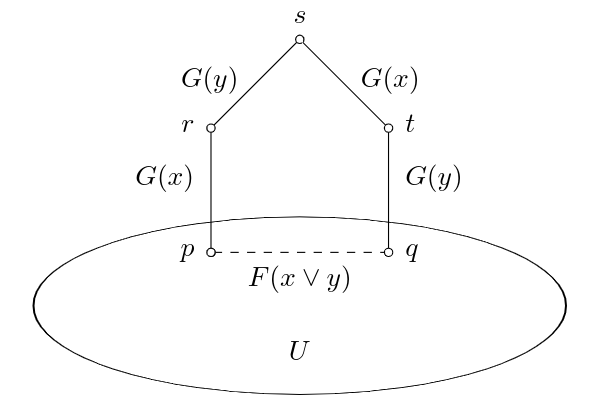
\includegraphics[scale=0.5]{./images/rel_lattice.png}
\end{center}
于是我们定义对任意的$z \in L$和$u,v \in U$, 使得$G(z)$满足下述条件
\begin{enumerate}
	\item $u~G(z)~v~\text{iff}~u~F(z)~v,$
	\item $u~G(z)~r~\text{iff}~z \geq x ~\text{and}~u~F(z)~p,$
	\item $u~G(z)~s~\text{iff}~z \geq x \vee y ~\text{and}~u~F(z)~p,$
	\item $u~G(z)~r~\text{iff}~z \geq y ~\text{and}~u~F(z)~p,$
	\item $r~G(z)~s~\text{iff}~z \geq y,$
	\item $s~G(z)~t~\text{iff}~z \geq x,$
	\item $r~G(z)~t~\text{iff}~z \geq x \vee y.$
\end{enumerate}
%TODO tikz!
注意到$G(z)$由于(1)是满足自反性的,并且满足了weak representtation上order关系,即$G(z) \cap U^2 = F(z)$. 同时观察到条件(2-7)都和$r,s,t$的位置无关,所以它们也都是满足对称性的. 传递性也是很显然的,i.e.,(2)(4) => (3) 和 (5)(6) => 7. 所以$G(z)$是一个等价关系. 还必须要说明$G$是单射和满足meet homomorphism. 由于$F$是单调,那么$G$肯定是单调,新加入的元素造成的relations不会对$G(x) \cap U^2 = F(x)$造成影响. 考虑$z,z' \in L$, 我们想要说明$G(z \wedge z') = G(z) \wedge G(z')$,其实就是要考虑$z,z'$和$x,y$的关系,记住若$z \wedge z' \geq x$当且仅当$z \geq x$和$z' \geq x$再结合上述条件,应该很容易证明,这过程太routine了! 我放弃了.

我们再来观察是否满足上述图里面的关系,首先来看$p~G(x)~r$, 把(2)中的$u$换成$p$和$z$换成$x$, 那么再看条件$x \geq x$ and $p~F(z)~p$, 这是显然满足的. 再来试一个$r~G(y)~s$,把(5)中的$z$换成$y$,那么条件变为$y \leq y$,这也是满足的. 回过头来看这个构造比较巧妙,注意到(2-4)必须带一个$u~F(x)~p$,这是要使得它们和$1$构成传递关系的时候是满足条件的.
\end{proof}

\begin{theorem}
\rm Every lattice has a type 3 representation.
\end{theorem}


\end{document}